\chapter{Research Framework\label{cha:method}}
%3100
The main purpose of this chapter is to describe a research approach used in this
study. The first section of the chapter identifies the objectives that need to
be addressed in order to achieve the goal of this study, followed by the research
questions in Section \ref{sec:questions} raised from these objectives.

Design Science Research (DSR) methodology was adopted by this study as the main
research methodology to address the research questions. This methodology
emphasizes the problem-solving and performance-improving paradigms and is
oriented towards creating and evaluating IT artifacts \citep{Hevner2004}. A
five-stage research project framework is outlined in Section \ref{sec:method}
which explains each stage of the project and the methods applied. Methodological
limitations are brought to considerations in Section \ref{sec:limits}. This
chapter concludes with the discussion of related work and projects carried out
in the area of \LLLsn.

\section{Research Objectives}

Understanding how \LLLs in universities can be effectively supported using
technical solutions is an overarching goal of this research. This goal brings up
a number of objectives that need to be addressed:
\begin{description}
  \item[Objective 1.] To determine student and institutional requirements for a
  \LLLs environment within the university context.
  \item[Objective 2.] To identify shortcomings and map these requirements
  against the systems already used in universities to support \LLLsn.
  \item[Objective 3.] To design and implement the features required in an
  environment that supports \LLLs to satisfy the defined requirements.
  \item[Objective 4.] To evaluate how this environment meets the needs of all
  stakeholders in supporting \LLLsn.
\end{description}

\section{Research Questions}
\label{sec:questions}
Based on the objectives, this study addressed the following research questions
supported by sub-questions:

\begin{description}
  \item[RQ1:] \textit{What is the concept of \LLLs and its connection to the
  universities?}
	\begin{itemize}
	  \item What is the role of \LLLs in the university context?
	  \item What is the motivation of universities in supporting \LLLsn?
  	  \item What are the existing university policies for supporting \LLLsn?
      \item What are the components of \LLLs environments in universities?
      \item What are the requirements for successful \LLLs support in
   universities?
	\end{itemize} 
	
   \item[RQ2:] \textit{How are available e-tools used to support \LLLs within
   the university context?}
	\begin{itemize}
		\item What e-tools are currently available to support \LLLsn:
			\begin{itemize}
				\item in general?
				\item in universities?
			\end{itemize}
		\item What are the conceptual strengths and weaknesses of these e-tools in
		university context?
		\item What is the relationship between LMS and e-tools support for \LLLs in
		university context?
	\end{itemize}

	\item[RQ3:] \textit{How can LMS and/or \ep~systems be extended to support
	students in a university context in \LLLsn?}
	\begin{itemize}
		\item What features are available now in these systems?
		\item What are the students and institutional requirements for LMS and
		\ep~to support \LLLsn?
		\item How can these requirements be translated and implemented into new or
		improved features?
	\end{itemize}

	\item[RQ4:] \textit{How does this extended environment meet the needs of the
	stakeholders in university teaching and learning contexts?}
	\begin{itemize}
		\item How can lecturers use new features to provide students with their
		guidance and help them to understand \LLLs skills?
		\item How can students address \LLLs skills using new features?
		\item How can new features help students track their learning progress, manage
		\ep~knowledge and content, demonstrate and share their achievements with
		others?
	\end{itemize}
\end{description}

\section{Research Approach}
\label{sec:method}

Finding the most efficient research approach is an important part of any
research study. A properly selected approach helps to obtain answers to the
research questions while working within the framework that uses methods that
have been verified and tested for validity \citep{Kumar2005}. Multi-paradigmatic
field of ICT offers a number of methodologies (e.g., theory building and
testing, action research, interpretive research, grounded theory, etc.) drawn
from the variety of research philosophies \citep{Vaishnavi2007}. This study
follows design science research methodology that has become popular over the
last five decades as fundamentally a problem-solving approach \citep{Cross1993}.

\subsection{Design Science Research Methodology}

According to \citet{Peffers2008}, design science research (DSR) originates from
engineering and computer science where design is a component of the research
process. \citet[p.~4]{Iivari2009} define DSR as \inlinequote{a research
activity that invents or builds new, innovative artifacts for solving problems
or achieving improvements}. Unlike software development methodology that
does not necessarily need any underlying theory, design science requires a
theoretical foundation for research \citep{Gero1999}. This approach is used in
ICT where there is a need to extend the existing boundaries of the current
systems or to address the important problems by creating new solutions and
artifacts \citep{Hevner2004}. The artifacts can be described as constructs
(vocabulary of a domain), methods (algorithms), models (abstractions),
instantiations (prototype systems), and better theories \citep{Hevner2010}. 

Requirements for DSR contribution, defined by \citet{March2008}, include (1)
identification of a problem, (2) demonstration that there are no existing
adequate solutions in the area, (3) development of an innovative artifact that
addresses the problem, (4) evaluation of the artifact, (5) communication of the
knowledge added to the area, and (6) understanding of the implications for
theory and practice.

This set of requirements closely resembles the DRS methodology process described
by \citet{Peffers2008} (see Figure \ref{fig:peffers}) and research model phases
found in \citet{Vaishnavi2007} (see Figure \ref{fig:vaishnavi}).

\begin{figure}[h!]
\centering
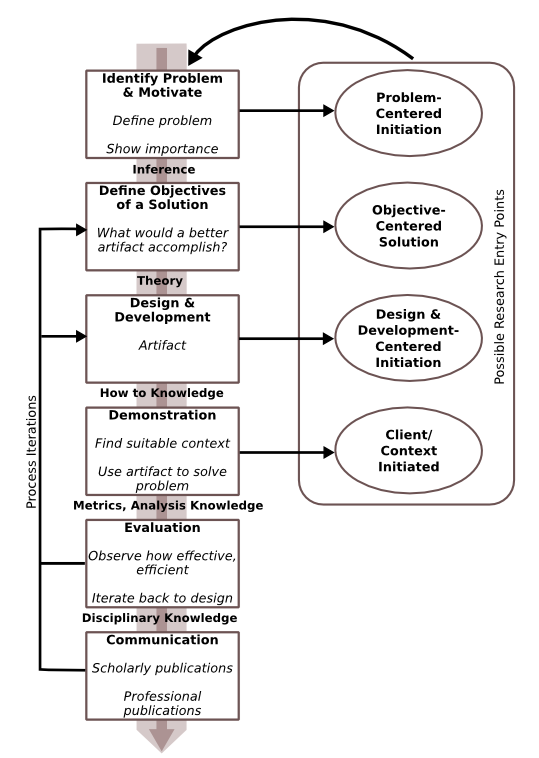
\includegraphics[height=0.76\textheight]{CH2-F1-Peffers}
\caption[Design Science Research Methodology Process Model]{Design Science
Research Methodology Process Model \citep{Peffers2008}}
\label{fig:peffers}
\end{figure}

\FloatBarrier

\begin{figure}[htp]
\centering
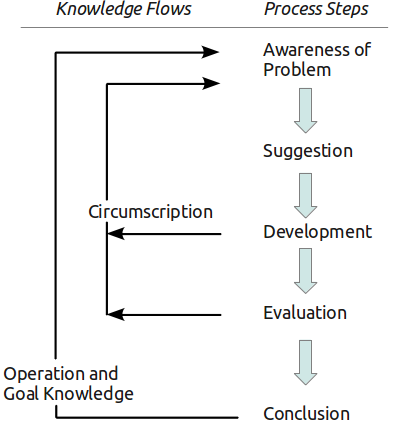
\includegraphics[width=0.5\textwidth]{CH2-F2-Vaishnavi}
\caption[Design Science Reseach Cycle]{Design Science Research Cycle
\citep{Vaishnavi2007}}
\label{fig:vaishnavi}
\end{figure}

All authors essentially agree on common elements. The initial stage of research
is \textit{problem identification} or \textit{awareness}, where a specific
research problem should be stated and the importance of its solution should be
justified. After the problem is identified, the next step is to \textit{suggest
a solution} and define its objectives. This includes understanding the state of
the problem and current available solutions, if any, and explaining how new
solution is going to address the problem in a better way. 

\FloatBarrier

The core phase of research is \textit{design and development}. Conceptually,
this phase consists of deciding the artifact's functional requirements or its
architecture and afterwards creating artifact itself. \citet{Peffers2008} note
that in some cases an artifact is not necessarily a new development. It might
have been already used in another research domain to solve a different problem.

Unlike Vaishnavi's research cycle where evaluation is one step of research
process, Peffer's model distinguishes between \textit{demonstration} and
\textit{evaluation} of the artifact. Demonstration is used to show that the
implemented idea works, while evaluation is more formal form of measuring how
well the artifact supports a solution to the problem \citep{Peffers2008}.
Artifact can be evaluated from various perspectives such as performance,
usability, reliability, accuracy, quality, functionality, etc.

The last stage of research is \textit{conclusion} or \textit{communication}. It
might involve but is not limited to: discussing the problem, its importance, the
novel artifact, and its effectiveness with relevant research audiences; creating
scholarly publications; presenting research findings at the conferences; and
writing a project report \citep{Archer1984}. However, if no satisfying results
have been reached at this stage of the research cycle, it might as well serve as
a subject for further research.

Described in Table \ref{tab:guidelines} are seven guidelines identified by
Hevner \citeyearpar{Hevner2004} that should be followed by the beginning
researches for effective DSR.

\begin{table}[htb]
  \caption[Design Science Research Guidelines]{Design Science Research
  Guidelines \citep{Hevner2004}}
  \begin{center}
    \begin{tabular}{| l | p{6.5cm} |}
    \hline
     \multicolumn{1}{|c|}{\textbf{Guidelines}} &
     \multicolumn{1}{c|}{\textbf{Description}} \\
     \hline
     Guideline 1: Design as an Artifact & Research must produce a viable
    artifact such as a construct, a model, a method or an instantiation \\ \hline
     Guideline 2: Problem Relevance & Research must develop technology-based
     solutions to important and relevant problems \\ \hline 
     Guideline 3: Design Evaluation & Proper valuation methods must be used to
     demonstrate artifact's quality and efficacy \\ \hline 
     Guideline 4: Research Contributions & Research must provide clear
     contributions to the research areas \\ \hline 
     Guideline 5: Research Rigor & Rigorous methods must be applied to
     construction and evaluation of the artifacts \\ \hline 
     Guideline 6: Design as a Search Process & Research must incorporate a
     search process to find and effective solution to the problem \\ \hline
     Guideline 7: Communication of Research & Research must be effectively
     communicated to relevant audiences \\ \hline
    \end{tabular}
  \end{center}
  \label{tab:guidelines}
\end{table}

In contrast to Hevner, \citet{Venable2010} argues that there is no common
understanding of what kind of guidelines and standards should be used for
effective DSR. However, based on analysis in the same work, the majority of
respondents who are researchers and DSR practitioners agree on a few points: DSR
should address important problems, have an artifact that would help to solve the
problem, and have some kind of evaluation of this artifact.

\subsection{Design Science Research Applied to This Project}

The research framework in the current research is adapted from a DSR cycle
established by \citet{Vaishnavi2007}. They identify five phases in the research
model: (a) identification of a problem, (b) suggestions and objectives of a
solution, (c) design and development, (d) demonstration and evaluation, and (e)
conclusion and communication.

Figure \ref{fig:path} shows a research path of this project from the first
to the last stage. It can be seen that at the later stages of the project it was
necessary to look back and reflect on findings in order to understand whether
the research objectives were met and what lessons were learnt. Other iterations
in this project were between stages three and two where the prototype had to be
taken back to the stakeholders for feedback. Although, according to Figures
\ref{fig:peffers} and \ref{fig:vaishnavi} the end of the evaluation can be
considered another potential stage to iterate back, \citet{Peffers2008} says
that the nature of the research project usually shows whether iterating back is
feasible or not. In this case, due to the time and resources constraints,
further improvements were left to subsequent projects.

\begin{figure}[htb]
\centering
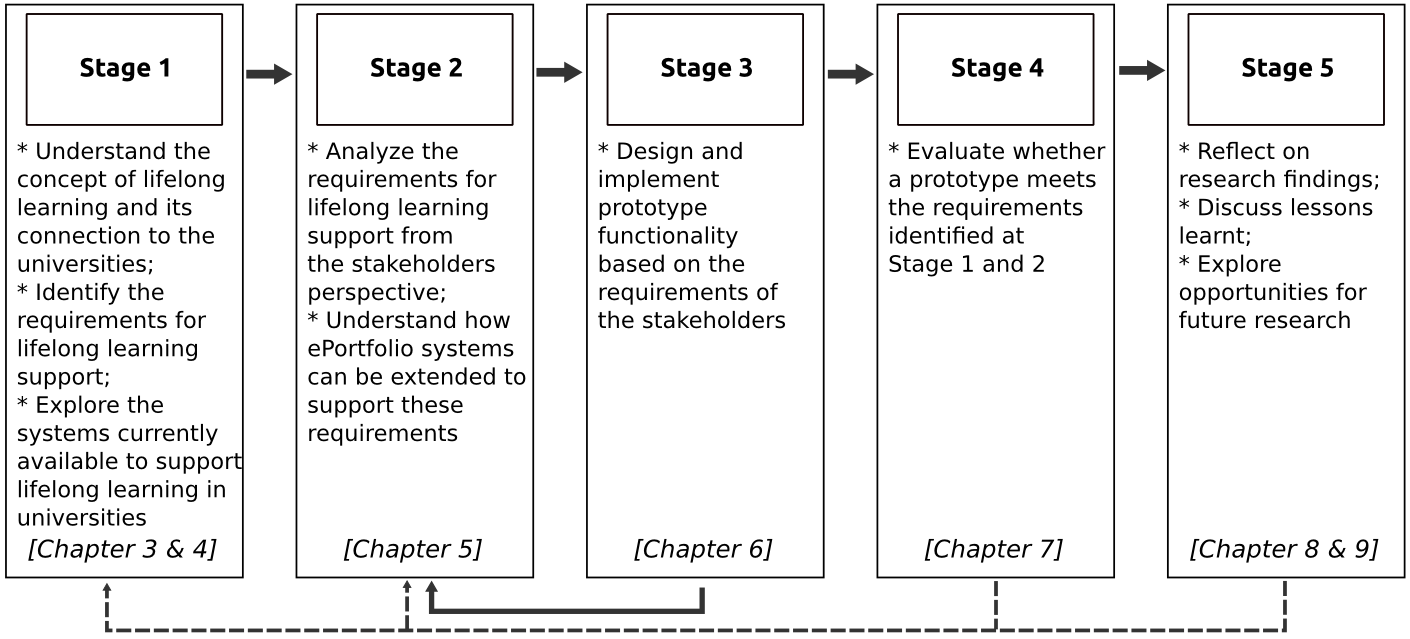
\includegraphics[width=1\textwidth]{CH2-F4-Path}
\caption{The research path}
\label{fig:path}
\end{figure}

\subsubsection{Stage 1. Problem Identification and Motivation}

Any research project can be started either from the gap in the literature or
when a problem that is worth solving exists \citep{Bourner2002}. Previous
experience and observations of the existing problems in the field of study
formed the background for this research. To define the main research topic,
preliminary investigations were made as part of the field of study review. The
problem identified in the current research is the difficulty in supporting
students' \LLLs in universities. Defining the research topic led to the research
questions and objectives development which, in turn, formed the direction and
focus of this project.

\subsubsection{Stage 2. Objectives of a Solution}

To answer the research question on the concept of \LLLs and what kind of
environment can support it, it is important to develop understanding of
current theories and practices of \LLLs support. A comprehensive literature
review and a review of the learning spaces was undertaken to address these
questions.

However, this research did not rely on a literature review alone. A set of
interviews with the stakeholders were organized to support literature findings
and identify the gaps that exist in current \ep~systems. Interviewees were
offered to look at the \ep~system from the \LLLs perspective and offer their
solutions for supporting guiding principles and recommendations for successful
\LLLs discovered in the literature.

Interviews were audio recorded, transcribed and analyzed. The results were
compiled into a set of formal software requirements specification to be
implemented in a system prototype for the future evaluations.

\subsubsection{Stage 3. Design and Development}

In the development phase, the results of the literature review, interviews and
requirements analysis were used to create a conceptual model of an \ep-supported
environment that can facilitate students in \LLLs and be compatible with
university needs.

A functionality, based on this model, was implemented in a prototype \ep~system.
As the requirements specification was too large for the project of such size and
relatively short timeline, only high priority requirements were implemented. The
requirements were prioritized according to the feedback given by the interviews
participants at the initial stages of the project. Due to this, a number of
requirements related to a better integration of the \ep~systems with LMS and
usability improvements were left behind. Although these requirements were not
implemented, they were still included into the conceptual model.

Prototyping followed established software engineering practices that interleaved
coding and revision, forming iterative development cycles, as it shown at Figure
\ref{fig:prototype}.

\begin{figure}[htb]
\centering
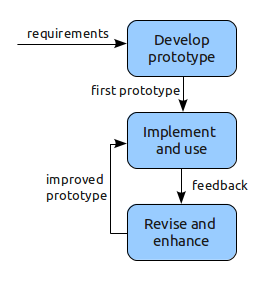
\includegraphics[height=0.3\textheight]{CH2-F3-Prototype}
\caption[Prototyping]{Prototyping based on \citet*[p.~411]{Sommerville2007}}
\label{fig:prototype}
\end{figure}

After each iteration was completed, the prototype was taken back to the
stakeholders for feedback. This was necessary to understand what changes were
required and to design further improvements. These iteration is shown on Figure
\ref{fig:path}.

Mahara \ep~system\footnote{\url{http://mahara.org}} was used as an initial base
system for the prototype. There is a number of reasons why this system was
selected. Mahara is a trusted and widely-used in universities (and at Massey
University in particular) solution with a large community support. This system
is open source which makes it easy to access and allows modifications like
adding new features and changing the existing ones. Mahara is a \textit{typical}
representative of its category and provides all commonly available features. At
the same time it is a leading edge system developed by using latest web
technologies and programming practice.

\subsubsection{Stage 4. Demonstration and Evaluation}

It is important for evaluation to be treated not as an isolated process, but as
a part of design process \citep{Cleven2009}. Although, the prototype was
reviewed by the stakeholders after every development cycle, a complex evaluation
of the overall concept was still required.

It is not likely that a single evaluation technique can establish effectiveness
and value of the prototype in a complex area of \LLLsn. In such cases it is
recommended \citep{Quinlan2008} that the evaluation design should incorporate a
variety of methods, that taken together can provide reasonable evaluation
outcomes.

Due to time and resources constraints, and an extended \ep~system being a
functional prototype, it was not feasible to conduct evaluations in the real
world settings. However, it was possible to develop a number of studies that
looked into the specific aspects of \LLLs support and evaluated how well
developed features satisfy the requirements identified earlier by the
stakeholders.
 
As a result, features implemented in the prototype were evaluated from three
different perspectives: 

\begin{itemize}
  \item Demonstrations of the prototype and its extended functionality were used
  for exploratory evaluation with the lecturers. The aim was to explore how the
  lecturers can integrate new features into their teaching to provide students
  with guidance and help them to understand \LLLs skills.
  
  \item An experiment with various representatives of undergraduate students
  was undertaken to understand how added functionality can help them to address
  institutional graduate attributes and \LLLs skills. Thirty five students with
  different levels of knowledge of \LLLs skills and experience of using
  \ep~systems were involved in the experiment.

  \item Case studies were used to evaluate prototype from the mature students
  perspective. This approach was selected due to its internal and external
  validity, control and in-depth examination of each case \citep{Yin2009}.
  Participant with a different study background had access to the prototype for
  an extended trial period of time and were able to get a better look at the new
  features. At the end of the trial period, each participant was interviewed and
  gave their feedback on the features they had used.
\end{itemize}

\subsubsection{Stage 5. Conclusion and Communication}

Where it was possible the results of the various stages of this research project
were documented and submitted for publications and conference presentations. Full
list of publications can be found in \hyperref[sec:pub]{Publications and
Presentations} section of this thesis.

\section{Methodological Limitations}
\label{sec:limits}

Any study and its findings should be weighed against methodological
limitations. Acknowledging limitations is important for scientific progress as
they might help to understand how research can be improved in the future
\citep{Ioannidis2007}. Although, literature does not explicitly describe
limitations of DSR methodology, they can still be derived from the limitations
of the methods used at each stage of the study. Therefore, the limitations
considered in this research included:

\begin{description}
\item[Sample size:] Sample size for Stage 2 was relatively small due to the
participants profile requirements. As well, snowballing sampling technique was
used to find suitable student participants which might have influences the
outcomes of this stage.
\item[Prototyping:] Evaluated system was a prototype based on open source
\ep~system Mahara which might have led to biased feedback as some participant
were familiar with the system and already had their opinion about it.
\item[Evaluation:] Due to the nature and scale of this research project, its
time and resources constraints, evaluation was not conducted in the real world
settings. Instead, a set of case studies, experiments and exploratory
evaluations have been undertaken.
\end{description}

More detailed discussion of the limitations can be found further in the relevant
chapters of this thesis.

\section{Related Work}
\label{sec:related}
As the field of \LLLs became popular, there were a number of studies aimed to
explore \LLLs support in various contexts. To date, research similar to this
project has not been identified, although projects found were a valuable source
of information and examples of previous research experience.

\begin{itemize}

  \item Lifelong Learning in London for
  All\footnote{\url{http://www.lkl.ac.uk/research/l4all.html}} (L4All): This
  project is focused on developing of \LLLs system to support independent
  learners (particularly those 16+ learners who traditionally have not
  participated in higher education) by recording their learning pathways. This
  project aimed to provide lifelong learners in the London region with access to
  information and resources that facilitates their progression from secondary
  education to further education or from secondary education directly to higher
  education \citep{Freitas2006};

  \item The Regional Interoperability Project on Progression for Lifelong
Learning\footnote{\url{http://www.nottingham.ac.uk/rippll}} (RIPPLL): This
project was going to establish a model of cross-sector collaboration in personal
development planning technology in the UK. The aim was to make all the major
existing electronic systems interoperable for study-based progress files that
are used in further and higher education to provide an easier transition process
from school to further education \citep{Hartnell-Young2006};

  \item ELGG-Moodle: In autumn 2006 Klagenfurt University, Austria was piloting
the project aimed to integrated Moodle LMS and ELGG platform. This integration
was used for professional development for all academic staff. Project outcomes
provided integration between systems such as single login and file transfer
\citep{Attwell2007}.

  \item Accessible \LLLc for Higher
  Education\footnote{\url{http://www.eu4all-project.eu}} (EU4ALL): A project
  started in 2006 and aimed to develop components and services for universities
  to make learning more accessible for both the students with functional
  diversity and the elderly. This project looked into providing a better access
  to the electronic content and educational resources in higher education using
  a framework or a set of free tools that support mobile learning, audio
  recording transcription, DAISY digital books and other adaptations of contents
  based on the student's needs and preferences.

  \item An \ep~based Pedagogy for Small to Medium-sized
  Enterprises\footnote{\url{http://www.wlv.ac.uk/ePPSME}} (ePPSME): Finished
  in 2011, this project provided higher education sector with reusable models
  for an \ep-based pedagogy for work-based learners. This pedagogy addresses
  the needs of learners with shortage of time, previous informal learning
  experience, need for flexible delivery and quality of learning, and
  opportunities to record achievements \citep{Felce2011}.
\end{itemize}

\section{Summary}

To address the objectives and research questions stated at the beginning of the
chapter, this research project follows DSR methodology. DSR is a problem solving
approach that focuses on development and evaluation of innovative IT artifacts.
This chapter outlined a five-stage research framework used in this work with
each stage explained.

The next chapter will explore the literature review undertaken to understand the
concept of \LLLs and the requirements for its efficient support. It will provide
a background for the further theory development of this research.
